\section{GPIO}
La periferica GPIO - General Purpose Input/Output ci permette di programmare alcuni pin del uC e di imporre un valore logico, oppure di leggere il valore logico che c'è su un pin.
Ci permettono in pratica di interfacciarci con il mondo esterno.

\subsection{Output}
\subsubsection{Direzione della corrente}
Configurati come output posso imporre il valore logico 1 oppure 0:
\begin{figure}[H]
    \centering
    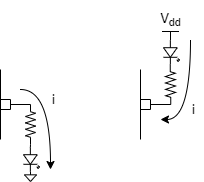
\includegraphics[width=150px]{images/21_GPIO/gpio_output_current.png}
\end{figure}
Se impongo 1 logico il pin può fornire corrente, infatti nel caso a sinistra quando poniamo 1 il led si accende.
Se impongo 0 logico il pin può assorbire corrente, infatti nel caso a destra quando poniamo 0 il led si accende. 

NB: Far passare la corrente nel senso contrario a quello previsto dal pin potrebbe danneggiare il componente, ad esempio se poniamo in uscita 1 logico ma all' altro capo del resistore poniamo 7V abbiamo che la corrente è in ingresso al pin, mentre dovrebbe essere in uscita.

\subsubsection{Struttura interna}
\begin{figure}[H]
    \centering
    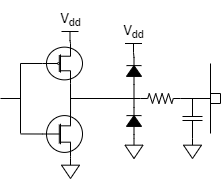
\includegraphics[width=150px]{images/21_GPIO/gpio_output_circuit.png}
\end{figure}
Il MOS in alto è un P-channel quello in basso è un N-channel.
Se chiudo il primo ed apro il secondo pongo 1 in uscita, se apro il primo e chiudo il secondo pongo 0 in uscita. 

NB: I due MOS non possono mai essere chiusi insieme, se succedesse avrei un cortocircuito nel chip e sarebbe dannoso.

I due diodi sono diodi di protezione, intervengono in caso la corrente all' interno del pin giri nel senso opposto a quello previsto canonicamente:
\begin{figure}[H]
    \centering
    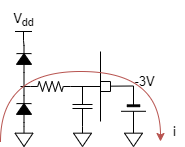
\includegraphics[width=150px]{images/21_GPIO/protection_diode.png}
\end{figure}
Hanno una certa tolleranza che ci può aiutare in caso di errore, tuttavia sono pensati per far si che le scariche elettrostatiche sui pin non danneggino l' interno del chip, sono infatti diodi anti-ESD (electrostatic discharge).

Il resistore in serie al pin è usata per evitare che carichi a bassa impedenza chiedano troppa corrente e danneggino i MOS, è current limiting resistor.

Il condensatore in parallelo all' uscita invece è un condensatore parassita, non è pertanto desiderato ma è presente per costruzione.

\subsubsection{Pilotare carichi}
Per pilotare carichi usando i GPIO conviene usare i livelli logici come ingresso per qualche amplificatore, banalmente dei transistori:
\begin{figure}[H]
    \centering
    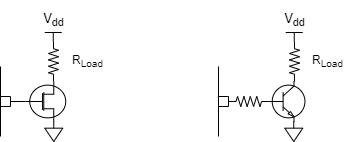
\includegraphics[width=250px]{images/21_GPIO/pilotare_carichi.png}
\end{figure}
Questo perché ogni pin può emettere al massimo 20mA ed in totale, tra tutti i pin come uscita, non si può emettere più di 200mA perché è la limitazione del pin di alimentazione del uC.

All' occorrenza potrebbe essere necessario però avere in uscita più di 20mA, ad esempio se vogliamo alimentare un LED in modo che si veda la sua luce anche di giorno bisogna dargli almento 30mA.
Possiamo pensare di usare 2 pin come uscita e sincronizzare il loro livello logico, in questo modo quando diamo livello alto su entrambe le uscite possiamo arrivare ad un massimo di 40mA:
\begin{figure}[H]
    \centering
    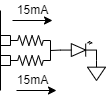
\includegraphics[width=100px]{images/21_GPIO/pin_in_parallelo_led.png}
\end{figure}
vediamo internamente cosa comporta questa connessione:
\begin{figure}[H]
    \centering
    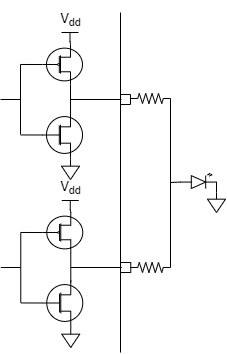
\includegraphics[width=150px]{images/21_GPIO/pin_in_parallelo_internal.png}
\end{figure}
Per far scorrere 30mA supponendo una caduta di tensione ai capi del led di $V_{\gamma} = 2.1V$:
$$ V_{R} = 5 - V_{\gamma} = 5-2.1 = 2.9V $$
$$ R = \frac{V}{I} = \frac{2.9V}{30mA} \approx 100 \Omega $$
quindi dobbiamo usare due resistori da 200$\Omega$ in modo che in parallelo diano 100$\Omega$.
Tutto questo ragionamento vale assumendo che la corrente arrivi in uguale misura da entrambi i pin, usando i MOS questa assunzione risulta vera perché se uno dei due rami fa scorrere più corrente porterà il MOS di quel ramo a riscaldarsi di più e quindi a condurre meno e dunque a trasportare meno corrente, si finisce quindi ad avere circa un pareggio.
Usando dei BJT invece questa assunzione non è vera perché i transistori bipolari con l' aumento della temperatura conducono di più, il che potrebbe portare al \emph{current hobbing}.

Devo fare attenzione ad ogni modo a non assegnare livello logico alto ad un pin e basso ad un altro pin perché crerei un corto circuito nell' alimentazione del uC, il che porterebbe a danneggiare i MOS o a scaricare l' eventuale batteria che alimenta il uC.
Le resistenze che abbiamo inserito possono aiutare anche in questa situazione poiché figurano come in serie ed abbiamo una limitazione alla corrente nel cortocircuito.
Un' altra soluzione è quella di inserire all' uscita dei pin dei diodi e la loro uscita inserirla in parallelo, in questo caso bisogna ricordare la caduta di tensione dei diodi.

Anche in caso usassi uscite di due uC diversi dovrei proteggerne almeno una con un resistore:
\begin{figure}[H]
    \centering
    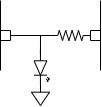
\includegraphics[width=100px]{images/21_GPIO/uscite_uC_diversi_in_parallelo.png}
\end{figure}
in questo caso si viene a creare una maglia RC con le capacità parassite, questo porta alla creazione di un limite superiore per la banda del sistema, quindi potrebbe rallentarlo.

\subsection{Input}
I pin possono anche essere configurati come ingresso.
Supponiamo di voler testare lo stato di un pulsante, possiamo usare i seguenti circuiti:
\begin{figure}[H]
    \centering
    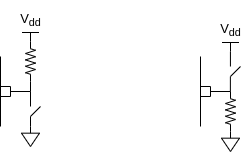
\includegraphics[width=200px]{images/21_GPIO/pull-up_pull-down.drawio.png}
\end{figure}
\begin{itemize}
    \item sulla sinistra abbiamo la confgiurazione con resistore in pull-up, quando il circuito è aperto e dunque il pulsante non è premuto abbiamo valore logico alto.
    Quando il pulsante è premuto sul pin abbiamo valore logico basso.
    
    \item sulla destra abbiamo la configurazione con resistore in pull-down, quando il circuito è aperto e dunque il pulsante non è premuto abbiamo valore logico basso.
    Quando il pulsante è premuto sul pin abbiamo valore logico alto.
\end{itemize}
In entrambi i casi il resistore si inserisce di valore alto in modo che la corrente che scorre in ingresso al pin sia piccola, però non deve neanche essere troppo alto perché la capacità parassita interna ha necessità di caricarsi e se la resistenza è troppo grande il tempo di caricamento anche è grande.
Per esempio: avendo $C = 10^{-11}F$ e $R=10^4 \Omega$ abbiamo che: $\tau = 10^{-11} \cdot 10^{4} = 10^{-7}s = 100 ns$
in questo caso il tempo di caricamento è trascurabile rispetto al clock.

Se non inserissi il resistore per fare pull-up/pull-down quando il circuito è chiuso ho un valore logico stabile, quando ce l' ho aperto il valore logico dipende da quanto è carica la capacità interna!

Il resistore di solito si inserisce di valore nel range di 10K - 47K.

\subsubsection{Struttura interna}
\begin{figure}[H]
    \centering
    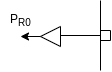
\includegraphics[width=150px]{images/21_GPIO/gpio_input_internals.drawio.png}
\end{figure}
Il buffer amplificatore legge il valore dall' esterno e permette al microcontrollore di leggerlo senza repentine modifiche della tensione.

Data questa struttura interna i pin sono più sicuri se impostati come input, possono essere messi in parallelo senza alcun problema.
Quando non vanno usati conviene sempre configurarli come ingresso, infatti al reset sono tutti impostati come pin di ingresso.

Si noti che i due circuiti di output ed input sono attivi allo stesso tempo, quindi i pin configurati come uscita possono comunque essere letti come ingresso:
\begin{figure}[H]
    \centering
    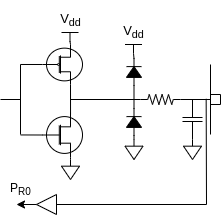
\includegraphics[width=175px]{images/21_GPIO/gpio_input_output.drawio.png}
\end{figure}

\subsubsection{Detect di un corto circuito tra i pin}
Dato che i pin possono essere configurati come uscita pur rimanendo come pin di ingresso possiamo usare questa feature per fare detecting di condizioni critiche:
\begin{figure}[H]
    \centering
    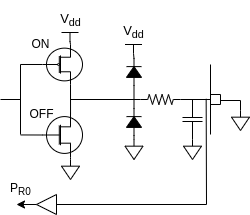
\includegraphics[width=200px]{images/21_GPIO/short_circuit_detection.png}
\end{figure}
essendo il MOS superiore chiuso ed il MOS inferiore spento abbiamo che l' uscita è impostata ad 1, tuttavia il pin è messo a ground.
Eseguendo una lettura del valore sul pin otteniamo infatti 0, siccome lo stato impostato in uscita è diverso da quello letto possiamo dire che c'è un cortocircuito sul pin.

Un problema del genere si ha anche quando ho due pin in parallelo ed ognuno ha in uscita un valore diverso, in tal caso il valore che vince il N-MOS e da lui il valore al canale.
Misuro le uscite e se sono diverse dal valore impostato come output allora abbiamo un cortocircuito.

\subsection{Registri}
I GPIO sono in totale 32 e sono divisi in gruppi da 8 in 4 batterie di registri diversi, ogni gruppo di 8 pin è detto \emph{porta}.
Abbiamo quindi:
\begin{itemize}
    \item Porta A: PA0, PA1, \_, PA7
    \item Porta B: PB0, PB1, \_, PB7
    \item Porta C: PC0, PC1, \_, PC7
    \item Porta D: PD0, PD1, \_, PD7
\end{itemize}

Ogni porta ha 3 registri di controllo e la posizione di ogni bit è riferita al pin che riguarda, es: il bit 0 dei registri di A riguardano tutti PA0,  

\subsubsection{DDRx}
E' il data direction register, se il bit è impostato ad 1 il pin è di uscita, se è a 0 il pin è di ingresso.

\subsubsection{PINx}
Se DDRx è impostato come input PINx indica il valore in ingresso su quel pin:
\begin{verbatim}
    IN r16, PINA
    ANDI r16, (1 << PA1)
\end{verbatim}

\subsubsection{PORTx}
Se DDRx è impostato come output in PORTx si inseriscono gli stati dei pin di uscita.
\begin{verbatim}
    LDI r16, (1 << PA0)
    OUT PORTA, r16
\end{verbatim}

\subsubsection{Pullup integrato}
C'è un resistore di pullup integrato per ogni pin, abbiamo la possibilità di abilitarlo e disabilitarlo a piacere.
Se il pin è impostato come input i bit di PORTx sono usati per indicare lo stato del pullup: 1 se deve essere abilitata, 0 se deve essere disabilitata.
Il resistore ha valore tra i 50k ed i 500k.

Inoltre il bit PUD (pull-up disable) può essere utilizzato per disabilitare globalmente i resistori di pull-up.

\subsubsection{Struttura interna}
\begin{figure}[H]
    \centering
    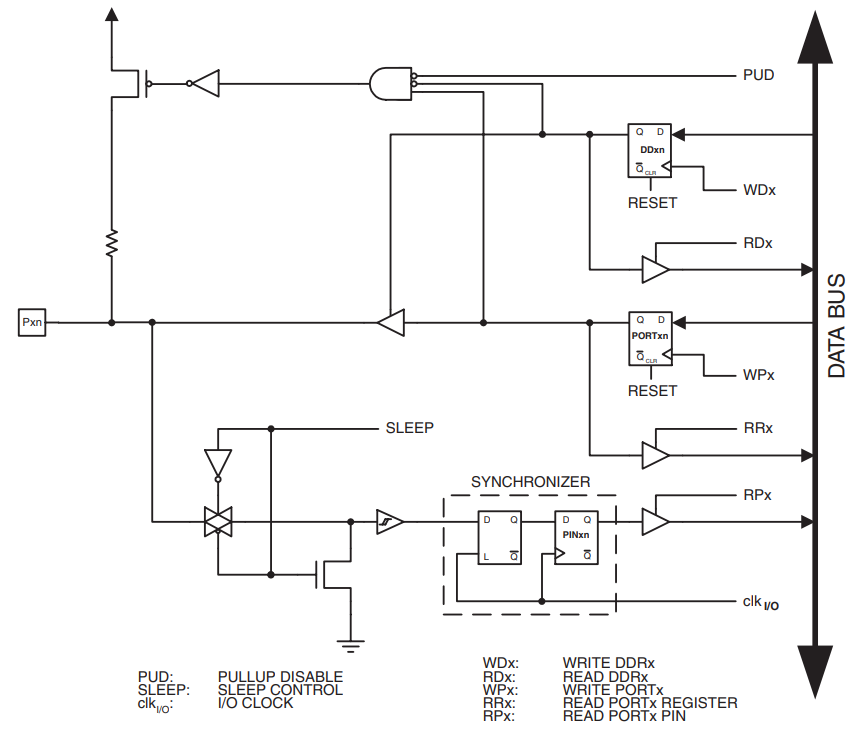
\includegraphics[width=330px]{images/21_GPIO/gpio_internal_structure.png}
\end{figure}
Quindi il resistore di pull-up è attivo se e solo se:
PUD = 0, DDRx = 0, PORTx = 1.

Per la lettura del valore in ingresso si usa un synchronizer per tenere stabile il valore di ingresso al flip flop di sampling perché il campionamento avviene all' atto della lettura del pin, non viene memorizzato periodicamente.

Si noti inoltre che prima del synchronizer vi è posto uno schmitt trigger.
Il valore in ingresso sul pin potrebbe non essere stabile al valore da campionare, anzi in genere oscilla abbastanza.
E' quindi necessario specificare per quale valore di tensione leggiamo 0 e per quale leggiamo 1, possiamo pensare di dividere il range della tensione con una soglia secca ma potrebbe essere problematico:
\begin{figure}[H]
    \centering
    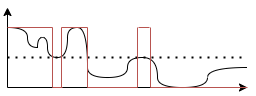
\includegraphics[width=250px]{images/21_GPIO/single_threshold.png}
\end{figure}
abbiamo una traduzione che risente molto delle oscillazioni del segnale.

Per risolvere il problema usiamo uno schmitt trigger cioè un comparatore con isteresi.
Si tratta di un comparatore con due soglie, superata la soglia superiore l' uscita è 1, superata la soglia inferiore l' uscita è 0 e nel mezzo tra le due soglie l' uscita rimane quella precedente.
Di seguito i diagrammi temporali dei due comparatori:
\begin{figure}[H]
    \centering
    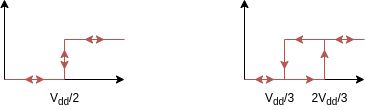
\includegraphics[width=250px]{images/21_GPIO/comparator_time_graphs.png}
\end{figure}

\subsubsection{Pin in comune}
Si noti che tutti i pin GPIO del uC sono in comune con qualche altra funzionalità:
\begin{figure}[H]
    \centering
    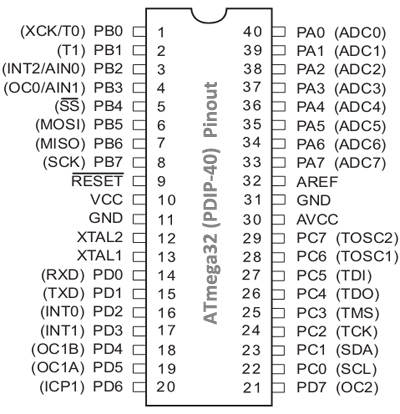
\includegraphics[width=200px]{images/21_GPIO/atmega32-pinout.jpg}
\end{figure}
